\documentclass[conference]{IEEEtran}
\usepackage{cite}
\usepackage{amsmath,amssymb,amsfonts}
\usepackage{algorithmic}
\usepackage{graphicx}
\usepackage{textcomp}
\usepackage{xcolor}
\usepackage{booktabs}
\usepackage{array}
\usepackage{colortbl}
\usepackage{pgfplots}
\usepackage{float}
\usepackage{dblfloatfix}
\usepackage{placeins}
% \usepackage{stfloats} 
\pgfplotsset{compat=1.18}

\definecolor{gapgreen}{RGB}{205,230,205}
\definecolor{gapred}{RGB}{240,205,205}
\definecolor{gapyellow}{RGB}{245,240,200}
\definecolor{gaporange}{RGB}{255,200,100}
\definecolor{gapblue}{RGB}{200,200,255}

\newcolumntype{R}[1]{>{\raggedright\arraybackslash}p{#1}}

\begin{document}

\title{Ingenier\'ia de Software Verde en Colombia frente a Europa, China y Am\'erica Latina: Una Revisi\'on Sistem\'atica de Literatura}

\author{\IEEEauthorblockN{J. C. Quintero Rubiano}
\IEEEauthorblockA{\textit{Grupo GNU/Linux de la Universidad Distrital (GLUD)}\\
\textit{Universidad Distrital Francisco Jos\'e de Caldas}\\
Bogot\'a, Colombia \\
jkquinteror@gmail.com}}

\maketitle

\begin{abstract}
La industria de las tecnolog\'ias de la informaci\'on representar\'a entre el 3\,\% y el 8\,\% de la demanda energ\'etica mundial para 2030, y los centros de datos por s\'i solos consumen el 1.8\,\% de la electricidad de Estados Unidos y generan cerca del 0.5\,\% de sus emisiones de gases de efecto invernadero, con proyecciones que anticipan un crecimiento de hasta 4.2 veces en sus emisiones globales para 2030. En Colombia, este imperativo adquiere un matiz adicional: la matriz el\'ectrica nacional es mayoritariamente hidroel\'ectrica y estructuralmente vulnerable a los ciclos de El Ni\~no--La Ni\~na, que alteran la generaci\'on de m\'as de un tercio de los embalses del mundo, por lo que la eficiencia energ\'etica del software se convierte en un asunto de seguridad energ\'etica. Esta Revisi\'on Sistem\'atica de Literatura (SLR), siguiendo PRISMA 2020 con fase de mapeo sistem\'atico Kitchenham/Petersen, 'sintetiza 35 art\'iculos indexados en Scopus, Google Scholar e IEEE Xplore para responder cu\'al es el estado actual de Green Cloud, Green DevOps y Green Software Engineering en Colombia comparado con Europa, China y Am\'erica Latina. La tesis del trabajo sostiene que Colombia posee capacidades t\'ecnicas aisladas y demostrables, pero carece de la pol\'itica p\'ublica, los est\'andares, la formaci\'on universitaria y la investigaci\'on aplicada longitudinal que permitan escalarlas. Los hallazgos evidencian cinco brechas cr\'iticas (pol\'iticas p\'ublicas, est\'andares t\'ecnicos, formaci\'on universitaria, investigaci\'on aplicada e infraestructura) y proponen siete recomendaciones con factores de \'exito para el contexto colombiano.
\end{abstract}

\begin{IEEEkeywords}
Ingenier\'ia de Software Verde, Revisi\'on Sistem\'atica de Literatura, Eficiencia Energ\'etica, Sostenibilidad del Software, Colombia, Am\'erica Latina
\end{IEEEkeywords}

\section{Introducci\'on}
El crecimiento exponencial de la infraestructura computacional ha consolidado la Ingenier\'ia de Software Verde como disciplina derivada del trabajo fundacional de Murugesan sobre Green IT~\cite{murugesan2008} y de los marcos de adopci\'on organizacional de Molla et al.~\cite{molla2009}. Informes ejecutivos estiman que los centros de datos representar\'an entre el 3\,\% y el 8\,\% de la demanda energ\'etica mundial para 2030~\cite{sanchez2023}, lo que convierte la sostenibilidad en un requisito de arquitectura y en un indicador de calidad fundamental en el ciclo de vida del software.

La evidencia emp\'irica reciente refuerza esta urgencia con datos medidos. Los centros de datos de Estados Unidos, que albergan cerca de una cuarta parte de los servidores del mundo, consumen alrededor del 1.8\,\% de la electricidad del pa\'is y generan aproximadamente el 0.5\,\% de sus emisiones de gases de efecto invernadero~\cite{siddik2021}. En el escenario m\'as adverso, las emisiones operativas de los centros de datos globales podr\'ian multiplicarse por 4.2 para 2030~\cite{maji2025}, superando la velocidad de descarbonizaci\'on de la red el\'ectrica. Este desacoplamiento entre el crecimiento de la demanda computacional y la descarbonizaci\'on de la red demuestra que la eficiencia de hardware y de fuente de energ\'ia no basta: el software debe volverse eficiente.

En el contexto colombiano, esta transici\'on enfrenta restricciones particulares. La matriz el\'ectrica de Colombia depende en m\'as de dos tercios de la generaci\'on hidroel\'ectrica, lo que la hace profundamente sensible a la variabilidad clim\'atica interanual. El fen\'omeno El Ni\~no--Oscilaci\'on del Sur (ENSO), la se\~nal clim\'atica interanual m\'as fuerte del planeta, altera significativamente la producci\'on anual de energ\'ia de m\'as de un tercio de los 1593 embalses estudiados, con impactos especialmente pronunciados en Sudam\'erica~\cite{ng2017}; el calentamiento global modifica la estad\'istica del ENSO~\cite{latif2009}, y el r\'ecord de calor de 2023 se ha atribuido en parte a la interacci\'on entre El Ni\~no y el calentamiento de fondo~\cite{karnauskas2025,columbia2016}. Bajo un super El Ni\~no, cae la generaci\'on renovable y sube la demanda por aire acondicionado, un doble estr\'es documentado para India con cerca de 18\,TWh de generaci\'on t\'ermica adicional~\cite{crea2026}. Los racionamientos hist\'oricos de 1992 y 2015--2016 en Colombia evidencian la materializaci\'on de este riesgo. Por lo tanto, la eficiencia energ\'etica del software en Colombia no es un lujo ambiental: es una pol\'itica de resiliencia energ\'etica.

A pesar de esta urgencia, el panorama nacional muestra capacidades t\'ecnicas aisladas sin infraestructura institucional: an\'alisis del costo energ\'etico de plataformas HPC/Grid~\cite{hernandez2011}, pol\'iticas de asignaci\'on energy-aware de m\'aquinas virtuales que reducen el consumo hasta en 30\,\%~\cite{diaz2013}, validaci\'on del modelo de madurez ISO/IEC 33000 para Green IT~\cite{paton2019}, marcos multicriterio para la ubicaci\'on de centros de datos en ciudades colombianas~\cite{torres2026} y casos sectoriales de software sostenible. Mientras tanto, Europa ha institucionalizado la sostenibilidad del software mediante la Green Software Foundation, regulaciones de eficiencia y la integraci\'on curricular~\cite{moreira2024}, y China ha incorporado criterios de eficiencia en sus est\'andares nacionales de TI y planes quinquenales~\cite{jin2025}. Am\'erica Latina avanza de forma m\'as lenta y fragmentada.

Este art\'iculo presenta una Revisi\'on Sistem\'atica de Literatura (SLR) siguiendo la metodolog\'ia PRISMA 2020 con fase de mapeo sistem\'atico (Kitchenham y Charters~\cite{kitchenham2007}; Petersen et al.~\cite{petersen2015}), con los siguientes objetivos: (1) mapear el estado actual de la investigaci\'on sobre Green Cloud, Green DevOps y Green Software Engineering; (2) establecer la tesis de que Colombia acumula evidencia t\'ecnica aislada pero carece de la infraestructura pol\'itica, normativa y formativa para escalarla; (3) identificar brechas entre la producci\'on global y la realidad colombiana; y (4) proporcionar insumos para la definici\'on de pol\'iticas y l\'ineas de investigaci\'on futuras.

\section{Trabajo Relacionado}
Revisiones previas han abordado la computaci\'on verde~\cite{harmon2009,rodriguez2022,sarasti2014} y las pr\'acticas de software sostenible~\cite{soto2022,currie2024}. La adopci\'on organizacional del Green IT ha sido modelada y validada~\cite{bustamante2014,cordero2022,molla2009}, y las evaluaciones t\'ecnicas de eficiencia de centros de datos en Am\'erica Latina incluyen enfriamiento free-cooling en Chile~\cite{diaz2017}, mini-servidores solares para educaci\'on rural en Per\'u~\cite{palomino2019} y c\'omputo m\'ovil distribuido de bajo costo~\cite{petrocelli2021}. Trabajos recientes sistematizan las perspectivas sobre pr\'acticas de software verde~\cite{miranda2025} y exploran el software verde para la gesti\'on, con el turismo como campo emergente~\cite{wu2025}. Los roadmaps de integraci\'on curricular~\cite{moreira2024,fontanarrosa2024} y los an\'alisis de pol\'itica nacional~\cite{bossa2023,rodriguezcorrea2023} completan el trasfondo de la comparaci\'on regional que se realiza aqu\'i.

\section{Metodolog\'ia}
La revisi\'on sigue el protocolo PRISMA 2020 complementado con una fase de mapeo sistem\'atico (Kitchenham y Charters~\cite{kitchenham2007}; Petersen et al.~\cite{petersen2015}).

\subsection{Estrategia de b\'usqueda}
La b\'usqueda se realiz\'o en cuatro fases: Fase 1 Scopus el 29--30 de agosto de 2026; Fase 2 IEEE Xplore la primera semana de septiembre de 2026; Fase 3 Google Scholar con optimizaci\'on Scholar Labs en septiembre de 2026; Fase 4 ACM Digital Library el 9 de septiembre de 2026. Las cadenas de b\'usqueda se definieron para reflejar el estado actual de la investigaci\'on y garantizar reproducibilidad.

Para Scopus e IEEE Xplore se utiliz\'o:
\texttt{TITLE-ABS-KEY((``green cloud'' OR ``green computing'' OR ``sustainable cloud'' OR ``green software engineering'' OR ``green devops'') AND (``Colombia'' OR ``Latin America''))}
con filtro de a\~no $PUBYEAR > 2010$.

Para Google Scholar:
\texttt{``green cloud'' OR ``green computing'' OR ``green software'' Colombia}

Los criterios de inclusi\'on cubrieron Green Cloud, Green DevOps, Green Software Engineering, sostenibilidad en TI y eficiencia energ\'etica de infraestructura computacional, con art\'iculos que aporten datos o discusi\'on sobre Colombia (Am\'erica Latina/Mercosur como contexto comparativo), en ingl\'es o espa\~nol.

\subsection{Flujo de selecci\'on}
La Tabla~\ref{tab:prisma} resume el flujo de selecci\'on PRISMA 2020. Tras la eliminaci\'on de duplicados, el cribado por t\'itulo y resumen y la evaluaci\'on de elegibilidad a texto completo, 35 estudios se incluyeron en la s\'intesis.

\begin{table}[H]
\caption{Flujo de selección PRISMA 2020}
\label{tab:prisma}
\centering
\footnotesize
\begin{tabular}{@{}R{3.5cm} R{1.0cm} R{3.5cm} @{}}
\toprule
\textbf{Etapa} & \textbf{N} & \textbf{Nota} \\
\midrule
Identificados (Scopus + Scholar + IEEE) & 135 & Registros iniciales \\
Duplicados eliminados & 7 & Elementos repetidos entre bases \\
Tras cribado & 128 & Filtro título/resumen \\
Excluidos en cribado & 92 & Fuera de criterios \\
Tras elegibilidad & 35 & Evaluación texto completo \\
Excluidos en elegibilidad & 1 & Criterios a texto completo \\
\textbf{Incluidos en la síntesis} & \textbf{35} & Estudios finales \\
\bottomrule
\end{tabular}
\end{table}

\subsection{Extracci\'on y clasificaci\'on de datos}
Despu\'es de la selecci\'on PRISMA se ejecut\'o una fase de mapeo en dos rondas: (1) extracci\'on de datos de tema, escenario de aplicaci\'on, instituci\'on principal, ciudad, metodolog\'ia, pa\'is, regi\'on y enfoque; y (2) clasificaci\'on emergente por tem\'atica TIC y escenario de aplicaci\'on, con tablas cruzadas y mapas tem\'aticos. Este h\'ibrido conserva el rigor de reporte PRISMA y la capacidad de s\'intesis visual propia del mapeo sistem\'atico.

Para el mapa regional se definieron cuatro categor\'ias mutuamente excluyentes. Colombia se trata como categor\'ia propia y se excluye de LAC (Am\'erica Latina y el Caribe) porque constituye el foco de an\'alisis de la revisi\'on: separarla habilita el an\'alisis de brechas entre Colombia y el resto de la regi\'on. LAC agrupa entonces los estudios de alcance latinoamericano sin Colombia. China se separa de la categor\'ia Global por su condici\'on de l\'ider con direcci\'on propia: su pol\'itica industrial, sus est\'andares de eficiencia y su formaci\'on universitaria avanzan de forma coordinada a escala nacional, un patr\'on estructuralmente distinto del resto del mundo; Global comprende los estudios de alcance mundial o de otras regiones sin China. La menor representaci\'on de estudios con alcance chino en la muestra inicial refleja la cobertura de las cadenas de b\'usqueda centradas en Colombia y Am\'erica Latina, no el volumen real de la producci\'on china, por lo que la b\'usqueda se ampli\'o con cadenas espec\'ificas para China y para el resto del mundo.

La Tabla~\ref{tab:hibrido} resume el mapeo entre las fases PRISMA 2020 y la fase de mapeo sistem\'atico.

\begin{table}[H]
\caption{Mapeo del protocolo h\'ibrido: fases PRISMA 2020 y fase de mapeo sistem\'atico}
\label{tab:hibrido}
\centering
\footnotesize
\begin{tabular}{@{}R{3.2cm} R{3.4cm} @{}}
\toprule
\textbf{Fase PRISMA 2020} & \textbf{Fase de mapeo (Kitchenham/Petersen)} \\
\midrule
Identificaci\'on y cribado & Definici\'on de preguntas y cadena de b\'usqueda \\
Elegibilidad a texto completo & Clasificaci\'on por relevancia tem\'atica \\
Inclusi\'on en la s\'intesis & Extracci\'on de metadatos (pa\'is, regi\'on, enfoque) \\
S\'intesis cualitativa & Tablas cruzadas y mapas tem\'aticos por escenario \\
Reporte y divulgaci\'on & Discusi\'on de brechas y recomendaciones \\
\bottomrule
\end{tabular}
\end{table}

\section{Resultados}
El corpus final de 35 estudios se caracteriza por tipo de fuente, regi\'on de procedencia (Colombia, Am\'erica Latina y el Caribe [LAC], Global y China) y enfoque metodol\'ogico (Figuras~\ref{fig:tiposfuente} y~\ref{fig:regiones}); la Tabla~\ref{tab:escenario-tema} cruza los escenarios de aplicaci\'on con los temas abordados por la literatura mapeada.

\begin{figure}[H]
\centering
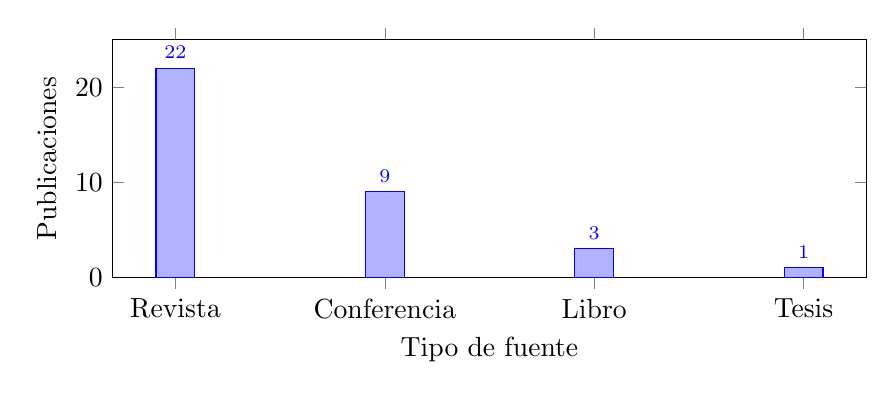
\begin{tikzpicture}
\begin{axis}[
ybar,
bar width=14pt,
width=0.92\columnwidth,
height=4.6cm,
symbolic x coords={Revista,Conferencia,Libro,Tesis},
xtick=data,
ymin=0, ymax=25,
ylabel={Publicaciones},
xlabel={Tipo de fuente},
nodes near coords,
nodes near coords style={font=\scriptsize}
]
\addplot coordinates {(Revista,22) (Conferencia,9) (Libro,3) (Tesis,1)};
\end{axis}
\end{tikzpicture}
\caption{Distribuci\'on de los 35 estudios incluidos por tipo de fuente.}
\label{fig:tiposfuente}
\end{figure}

\begin{figure}[H]
\centering
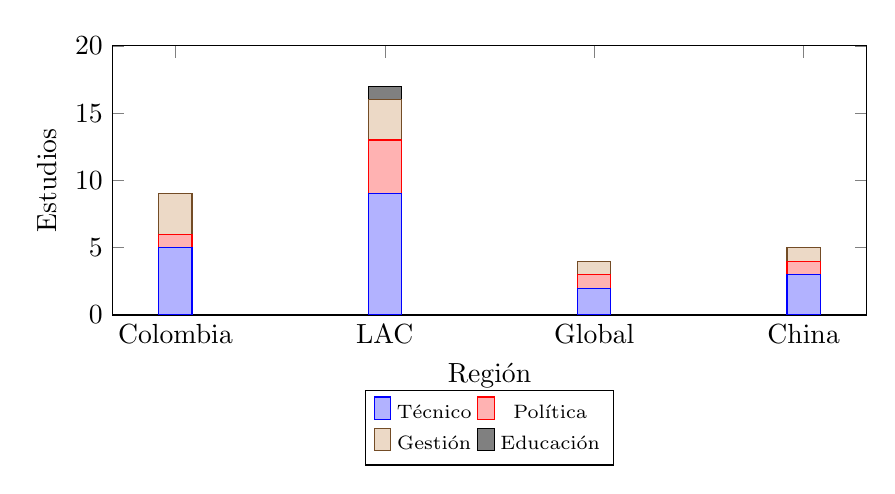
\begin{tikzpicture}
\begin{axis}[
ybar stacked,
bar width=12pt,
width=0.92\columnwidth,
height=5cm,
symbolic x coords={Colombia,LAC,Global,China},
xtick=data,
ymin=0, ymax=20,
ylabel={Estudios},
xlabel={Regi\'on},
legend style={at={(0.5,-0.28)},anchor=north,legend columns=2,font=\scriptsize},
legend entries={T\'ecnico,Pol\'itica,Gesti\'on,Educaci\'on}
]
\addplot coordinates {(Colombia,5) (LAC,9) (Global,2) (China,3)};
\addplot coordinates {(Colombia,1) (LAC,4) (Global,1) (China,1)};
\addplot coordinates {(Colombia,3) (LAC,3) (Global,1) (China,1)};
\addplot coordinates {(Colombia,0) (LAC,1) (Global,0) (China,0)};
\end{axis}
\end{tikzpicture}
\caption{Estudios incluidos por regi\'on y enfoque metodol\'ogico ($n=35$). LAC: Am\'erica Latina y el Caribe.}
\label{fig:regiones}
\end{figure}

\FloatBarrier
\begin{table}[H]
\caption{N\'umero de publicaciones por escenario de aplicaci\'on (filas) y tema (columnas), $n=35$}
\label{tab:escenario-tema}
\centering
\scriptsize
\resizebox{\columnwidth}{!}{%
\begin{tabular}{@{}l R{1cm} R{1cm} R{1cm} R{1cm} R{1cm} R{0.7cm} @{}}


\toprule
\textbf{Escenario} & \textbf{GSE} & \textbf{Green IT/GC} & \textbf{Cloud} & \textbf{DC} & \textbf{Pol\'itica/ Gesti\'on} & $\Sigma$ \\
\midrule
Empresa y organizaciones & 0 & 3 & 0 & 0 & 4 & 7 \\
Centros de datos & 0 & 0 & 0 & 6 & 1 & 7 \\
Cloud y virtualizaci\'on & 1 & 0 & 5 & 0 & 0 & 6 \\
Desarrollo y operaciones de software & 4 & 0 & 0 & 0 & 0 & 4 \\
Educaci\'on & 0 & 1 & 0 & 0 & 1 & 2 \\
Otros sectores & 1 & 5 & 1 & 0 & 2 & 9 \\
\midrule
$\Sigma$ & 6 & 9 & 6 & 6 & 8 & 35 \\
\bottomrule
\end{tabular}
}
\end{table}

\subsection{Dimensiones t\'ecnicas y m\'etricas}
Los 35 art\'iculos coinciden en que las m\'etricas operativas son la puerta de entrada para la adopci\'on de pr\'acticas verdes. El \'indice SCI (Software Carbon Intensity) de la Green Software Foundation es el est\'andar m\'as citado para medir emisiones por unidad funcional~\cite{fontanarrosa2024,jin2025}, mientras que la m\'etrica PUE (Power Usage Effectiveness) sigue siendo el referente para evaluar la eficiencia de centros de datos, con valores cercanos a 1.0 que indican m\'axima eficiencia frente a 2.0 o m\'as en infraestructuras sin optimizar~\cite{harmon2009,diaz2017}.

La evidencia contextual reciente ampl\'ia el marco m\'etrico en tres dimensiones. Primero, del PUE al carbono total del ciclo de vida: la especializaci\'on de hardware mejora la eficiencia operativa pero incrementa las emisiones incorporadas, motivando m\'etricas unificadas como el Job Sustainability Cost y el Amortized Sustainability Cost~\cite{eilam2024}; para Colombia, la estrategia de adquirir hardware m\'as eficiente debe evaluarse contra la prolongaci\'on del ciclo de vida. Segundo, del Scope 2 al alcance completo de la cadena: entre el 38\,\% y el 69\,\% del carbono total de un centro de datos corresponde a emisiones de Scope 3~\cite{lin2024}, lo que refuerza la necesidad de m\'etricas de ciclo de vida. Tercero, de la energ\'ia al agua como recurso contable: el enfriamiento seco puede reducir el consumo de agua de un centro de datos hasta en 4.34 millones de galones al mes, aunque los trade-offs dependen de la geograf\'ia~\cite{gnibga2024}; en un pa\'is con estr\'es h\'idrico estacional como Colombia, esta dimensi\'on no debe ignorarse en la ubicaci\'on de infraestructura.

Hallazgos t\'ecnicos transversales: la prolongaci\'on del ciclo de vida de servidores reduce significativamente la tasa de emisi\'on amortizada anual; la consolidaci\'on en la nube multi-inquilino evita la capacidad ociosa~\cite{rodriguez2022,petrocelli2021}; migrar infraestructura de TI tradicional a la nube reduce las emisiones de carbono entre el 72\,\% y el 98\,\%~\cite{microsoft2020}; el desplazamiento temporal y geogr\'afico de cargas intensivas seg\'un la intensidad de carbono de la red es viable pero escasamente implementado en la regi\'on~\cite{bellal2026,lozoya2022}; y las herramientas de observabilidad energ\'etica requieren validaci\'on rigurosa, pues Kepler sobreestima el consumo hasta en 15$\times$~\cite{bellal2026}.

La evidencia colombiana incluye: an\'alisis del costo energ\'etico por estados idle/active y transferencia de datos en plataformas HPC/Grid~\cite{hernandez2011}; pol\'iticas de asignaci\'on energy-aware de m\'aquinas virtuales que reducen el consumo hasta en 30\,\%~\cite{diaz2013}; validaci\'on de la familia ISO/IEC 33000 para gobernanza y madurez de Green IT~\cite{paton2019}; y un marco multicriterio que identifica a Bogot\'a y Medell\'in como las ciudades m\'as aptas para la ubicaci\'on de centros de datos~\cite{torres2026}.

\subsection{Brechas de pol\'itica y formaci\'on}
Un hallazgo cr\'itico y consistente es la ausencia de pol\'iticas nacionales estructuradas para la sostenibilidad del software en Colombia~\cite{bossa2023,rodriguezcorrea2023}. Mientras la Green Software Foundation ha establecido una meta de reducci\'on del 45\,\% de emisiones para 2030~\cite{sanchez2023} y China integra criterios verdes en sus est\'andares nacionales~\cite{jin2025}, la evidencia reciente muestra que los pilotos nacionales de centros de datos verdes en China mejoran la eficiencia energ\'etica empresarial mediante mecanismos de \textit{green empowerment} y \textit{data empowerment}~\cite{wangHowCanNational2026}. Modelos bi-nivel para cl\'usteres de centros de datos acoplan c\'omputo y electricidad y permiten aumentar el uso de renovables 1.18\,\% con una reducci\'on de costo total de 5.43\,\%~\cite{zhangBilevelPlanningModel2026}. En construcci\'on, la aglomeraci\'on industrial presenta una relaci\'on en U invertida con la productividad total de factores verdes, moderada al alza por servicios de consultor\'ia~\cite{wangNonlinearImpactIndustrial2026}. Colombia muestra: (1) ausencia de pol\'itica p\'ublica obligatoria que incentive o exija pr\'acticas de software verde, dejando la responsabilidad al criterio voluntario de las empresas~\cite{rodriguezcorrea2023,bustamante2014}; (2) falta de est\'andares obligatorios, a diferencia de Europa donde el dise\~no ecol\'ogico de software comienza a regularse~\cite{miranda2025,puerta2024}; y (3) brecha de formaci\'on, con m\'odulos escasos o nulos de sostenibilidad en los programas de ingenier\'ia de software colombianos y solo el 13.5\,\% de las universidades consideradas eficientes energ\'eticamente~\cite{castro2025,puerta2024}, mientras existe un roadmap curricular validado~\cite{moreira2024}. El caso EducaAmbienteWeb demuestra potencial aislado en la gesti\'on de residuos electr\'onicos sin proyecci\'on nacional~\cite{botero2023}.

\subsection{Aplicaciones y casos de uso}
Las aplicaciones documentadas incluyen: optimizaci\'on de infraestructura de centros de datos (PUE, consolidaci\'on en nube, gesti\'on de carbono incorporado)~\cite{garcia2022,torres2026,diaz2017}; educaci\'on ambiental con mini-servidores solares que reducen el consumo 23$\times$ en Per\'u~\cite{palomino2019}; principios de desarrollo de software verde y herramientas de medici\'on SCI en proyectos piloto~\cite{miranda2025,jin2025}; transferencia de tecnolog\'ias verdes desde Corea y Europa hacia Am\'erica Latina~\cite{piaggesi2019,cordero2022}; y c\'omputo m\'ovil distribuido de bajo costo sobre dispositivos ARM~\cite{petrocelli2021}.

\subsection{Software verde para gesti\'on y turismo}
Wu et al.~\cite{wu2025}, mediante un enfoque h\'ibrido (bibliom\'etrico + SLR) sobre Web of Science (1991--2024), confirman que el turismo aparece marginalmente en el software verde y ofrece oportunidades prometedoras. Para Colombia, donde el turismo es un sector econ\'omico estrat\'egico (ecoturismo del eje Cafetero, Cartagena, Leticia), la intersecci\'on entre software verde y turismo permanece inexplorada en los 35 art\'iculos incluidos, lo que representa una oportunidad concreta de investigaci\'on.

\subsection{Matriz comparativa regional}
La Tabla~\ref{tab:comparativa} transpone la comparaci\'on regional en filas de regiones y columnas de dimensiones operativas, seg\'un la clasificaci\'on del mapeo sistem\'atico. La Tabla~\ref{tab:gaps} presenta una matriz de brechas donde el verde indica dimensi\'on presente, el amarillo indica presencia parcial y el rojo indica ausencia.

\FloatBarrier
\begin{table}[H]
\caption{Comparaci\'on regional: pol\'itica, formaci\'on y m\'etricas}
\label{tab:comparativa}
\centering
\scriptsize
\resizebox{\columnwidth}{!}{%
\begin{tabular}{@{}R{1.2cm} R{3.6cm} R{3.4cm} R{3.8cm} @{}}


\toprule
\textbf{Regi\'on} & \textbf{Pol\'itica y est\'andares} & \textbf{Formaci\'on universitaria} & \textbf{M\'etricas y casos} \\
\midrule
\textbf{Colombia} & Ausente: no existe pol\'itica ni est\'andares obligatorios~\cite{bossa2023,rodriguezcorrea2023} & M\'odulos aislados o nulos; 13.5\,\% de universidades eficientes~\cite{castro2025,puerta2024} & Casos aislados (UIS, Uniandes, Univalle); sin estudios longitudinales~\cite{hernandez2011,diaz2013,paton2019} \\
\textbf{Europa} & Green Software Foundation; regulaciones de eficiencia~\cite{sanchez2023} & Integraci\'on curricular estudiada y en curso~\cite{moreira2024,fontanarrosa2024} & Amplia adopci\'on de PUE/SCI; casos empresariales y acad\'emicos~\cite{harmon2009,diaz2017} \\
\textbf{China} & Planes quinquenales con metas de carbono del sector digital~\cite{jin2025} & M\'odulos de software verde en planes de ingenier\'ia~\cite{jin2025} & Adopci\'on a escala nacional impulsada por est\'andares~\cite{jin2025} \\
\textbf{LatAm\slash Mercosur} & Fragmentada, iniciativas aisladas~\cite{bossa2023} & Similar o peor que Colombia~\cite{puerta2024} & Emergente, mayormente investigaci\'on; caso de mini-servidor solar en Per\'u~\cite{palomino2019} \\
\bottomrule
\end{tabular}
}
\end{table}

\begin{table}[H]
\caption{Matriz de brechas Colombia: capacidad t\'ecnica vs. infraestructura institucional}
\label{tab:gaps}
\centering
\footnotesize
\begin{tabular}{@{}R{1.5cm} R{1.8cm} R{1.8cm} R{2.0cm} @{}}
\toprule
\textbf{Dimensi\'on} & \textbf{Capacidad t\'ecnica} & \textbf{Infraestructura institucional} & \textbf{Evidencia clave} \\
\midrule
Pol\'itica & \cellcolor{gapyellow}Embrionaria & \cellcolor{gapred}Ausente & Sin marco normativo obligatorio~\cite{bossa2023,rodriguezcorrea2023} \\
Formaci\'on & \cellcolor{gaporange}Parcial & \cellcolor{gapred}Ausente & M\'odulos aislados, 13.5\,\% universidades eficientes~\cite{castro2025,puerta2024} \\
Investigaci\'on aplicada & \cellcolor{gapgreen}Presente & \cellcolor{gapred}Ausente & Casos UIS/Uniandes, sin seguimiento longitudinal~\cite{hernandez2011,diaz2013,paton2019} \\
M\'etricas y reporte & \cellcolor{gaporange}Parcial & \cellcolor{gapred}Ausente & Uso de PUE/SCI piloto, sin reporte obligatorio~\cite{fontanarrosa2024,jin2025} \\
\bottomrule
\end{tabular}
\end{table}

La secci\'on IV-A tambi\'en destaca que el c\'alculo del \'indice SCI requiere datos de energ\'ia consumida, intensidad de carbono de la red, carbono incorporado del hardware y una unidad funcional~\cite{fontanarrosa2024}. Para organizaciones con recursos limitados, herramientas de c\'odigo abierto como CloudCarbonFootprint y GREENER permiten estimar estas m\'etricas sin instrumentaci\'on profunda~\cite{currie2024}. En contextos de PYMES colombianas, se recomienda iniciar con el c\'alculo de PUE en infraestructura de servidores locales~\cite{garcia2022} y avanzar hacia SCI cuando la madurez de procesos lo permita.

La Tabla~\ref{tab:citas} lista las publicaciones del corpus con mayor impacto citacional verificado.

\begin{table}[H]
\caption{Publicaciones m\'as citadas relacionadas con la revisi\'on (Google Scholar/ACM DL, septiembre de 2026)}
\label{tab:citas}
\centering
\footnotesize
\begin{tabular}{@{}R{4.7cm} R{1.3cm} R{0.9cm} @{}}
\toprule
\textbf{Publicaci\'on (a\~no)} & \textbf{Tipo} & \textbf{Citas} \\
\midrule
Harmon y Auseklis (2009), servicios TI sostenibles & corpus & 146 \\
Moreira et al. (2024), roadmap de educaci\'on & referencia & 26 \\
De Micco et al. (2020), sistemas embebidos en Latinoam\'erica & corpus & 18 \\
Wu et al. (2025), software verde y turismo & corpus & 2 \\
Piaggesi et al. (2019), transferencia Corea--Colombia & corpus & 0 \\
\bottomrule
\end{tabular}
\end{table}

\section{Discusi\'on}
\subsection{Interpretaci\'on de resultados}
La s\'intesis de los 35 art\'iculos revela un patr\'on claro: la investigaci\'on t\'ecnica sobre software verde existe y acumula m\'etricas y herramientas operativas, pero la infraestructura de pol\'itica, est\'andares y formaci\'on que permite la adopci\'on a escala est\'a ausente en Colombia~\cite{bossa2023}. Esto genera una brecha de conocimiento y aplicaci\'on donde los avances t\'ecnicos aislados no se traducen en cambios sist\'emicos. Los hallazgos t\'ecnicos son transferibles y adoptables de inmediato por organizaciones colombianas, pero la escalabilidad requiere tres condiciones actualmente ausentes: pol\'iticas que incentiven la medici\'on y el reporte, est\'andares que eleven la sostenibilidad a requisito de dise\~no y curr\'iculos universitarios que formen a los pr\'oximos ingenieros en principios verdes.

\subsection{Vulnerabilidad energ\'etica como argumento de urgencia}
La evidencia clim\'atico-energ\'etica incorporada en esta revisi\'on a\~nade una dimensi\'on propia. Colombia genera m\'as de dos tercios de su electricidad con hidroel\'ectricas. El ENSO altera significativamente la producci\'on anual de m\'as de un tercio de los embalses del mundo, con efectos especialmente pronunciados en Sudam\'erica~\cite{ng2017}; en t\'erminos agregados globales las anomal\'ias se cancelan, pero a escala nacional y de cuenca los efectos son severos. El calentamiento global modifica la estad\'istica del ENSO~\cite{latif2009}, y el r\'ecord de calor de 2023 se ha atribuido en parte a la interacci\'on ENSO--calentamiento~\cite{karnauskas2025,columbia2016}. Para un sistema como el colombiano, cada ciclo de El Ni\~no implica riesgo de sequ\'ia en los embalses, ca\'ida de generaci\'on y presi\'on sobre la demanda por calor, exactamente el patr\'on doble documentado para India con cerca de 18\,TWh de generaci\'on t\'ermica adicional~\cite{crea2026}.

Esta cadena (ENSO $\rightarrow$ hidrolog\'ia $\rightarrow$ mix de generaci\'on $\rightarrow$ intensidad de red $\rightarrow$ demanda de software) se presenta como hip\'otesis contextual externa al corpus de la SLR, con salvedades expl\'icitas: las cifras de Estados Unidos~\cite{siddik2021} no son directamente extrapolables a Am\'erica Latina; la proyecci\'on de 4.2 veces~\cite{maji2025} es un escenario, no un resultado determinista; y el corpus de 35 art\'iculos limita la fuerza de cualquier generalizaci\'on regional. Si la generaci\'on el\'ectrica es escasa y estresada en los picos de demanda, cada kWh ahorrado por software eficiente es un kWh que no compite con los servicios esenciales, posicionando el software eficiente como amortiguador de demanda en los momentos m\'as cr\'iticos del sistema el\'ectrico. Este argumento eleva el estudio m\'as all\'a del cumplimiento ambiental: lo posiciona como insumo de pol\'itica de resiliencia energ\'etica nacional, un marco ausente en la literatura colombiana mapeada y una contribuci\'on de esta revisi\'on.

\subsection{Brechas identificadas en la investigaci\'on colombiana}
Emergen cinco brechas consistentes: (1) de pol\'itica, sin pol\'itica p\'ublica que obligue o incentive la sostenibilidad del software, la m\'as cr\'itica, pues la acci\'on voluntaria ser\'a insuficiente~\cite{maji2025}; (2) de est\'andares, sin est\'andares t\'ecnicos ni mecanismos de certificaci\'on, lo que deja invisibles las emisiones de Scope 3 (38\,\%--69\,\% del carbono de un centro de datos~\cite{lin2024}) y el carbono incorporado~\cite{eilam2024}; (3) de formaci\'on, con contenidos casi nulos de sostenibilidad en los programas de ingenier\'ia de software, abordable mediante el roadmap curricular importable~\cite{moreira2024}; (4) de investigaci\'on aplicada, dominada por estudios te\'oricos o casos aislados sin medici\'on longitudinal de impacto; y (5) de infraestructura, con pocos art\'iculos que aborden la optimizaci\'on espec\'ifica colombiana y sin inventario p\'ublico de la huella energ\'etica de los centros de datos del pa\'is, pese a los trade-offs documentados~\cite{gnibga2024,torres2026}.

\subsection{Limitaciones}
La composici\'on del corpus sesga hacia lo t\'ecnico (19 de 35 art\'iculos), por lo que las afirmaciones sobre pol\'itica y formaci\'on descansan en un subconjunto minoritario y deben leerse como evidencia exploratoria. La b\'usqueda abarc\'o Scopus, IEEE Xplore, ACM Digital Library y Google Scholar; no obstante, no se identificaron estudios con afiliaci\'on colombiana en ACM en la ventana revisada, lo que refuerza la escasez de producci\'on local. La revisi\'on fue liderada por un autor y careci\'o de validaci\'on inter-rater, por lo que los criterios de inclusi\'on se documentan de forma expl\'icita para reproducibilidad. Solo se incluyeron art\'iculos en ingl\'es o espa\~nol, excluyendo contribuciones en chino y portugu\'es; la b\'usqueda se cerr\'o en agosto de 2026. El an\'alisis es cualitativo y de s\'intesis, no un meta-an\'alisis cuantificado. Las fuentes clim\'atico-energ\'eticas son contextuales y no forman parte del corpus PRISMA; su selecci\'on fue dirigida y su uso como marco contextual es expl\'icito. Este trabajo se enmarca como mapeo exploratorio inicial y no pretende generalizaciones definitivas del estado del arte mundial.

\section{Conclusiones}
La revisi\'on confirma una brecha sustancial entre la producci\'on global de conocimiento en Ingenier\'ia de Software Verde y la realidad de investigaci\'on y adopci\'on en Colombia. Mientras el mundo avanza en la integraci\'on de m\'etricas (SCI, PUE, carbono incorporado), pol\'iticas (Green Software Foundation, regulaciones europeas y chinas) y formaci\'on universitaria~\cite{moreira2024,jin2025}, Colombia presenta un escenario de desarrollo t\'ecnico aislado sin la infraestructura pol\'itica ni institucional que permita la adopci\'on escalada. La tesis del trabajo, Colombia tiene capacidades t\'ecnicas demostrables pero no escalables por la ausencia de pol\'itica, est\'andares y formaci\'on, se confirma con los 35 art\'iculos mapeados y se refuerza con la evidencia contextual: la urgencia no es solo ambiental, es de seguridad energ\'etica nacional, dado el peso de la hidroelectricidad y la vulnerabilidad al ENSO~\cite{ng2017,crea2026,latif2009}.

Se proponen siete recomendaciones con factores de \'exito: (1) una pol\'itica nacional de sostenibilidad en TI del Ministerio de Tecnolog\'ias de la Informaci\'on y las Comunicaciones, enmarcada como instrumento de resiliencia energ\'etica y con metas medibles faseadas; (2) est\'andares t\'ecnicos colombianos de software verde en colaboraci\'on con la Green Software Foundation, incluyendo reporte de Scope 3 y carbono incorporado~\cite{lin2024,eilam2024}; (3) m\'odulos obligatorios en los planes de estudio universitarios (m\'inimo 40 horas transversales) siguiendo el roadmap de Moreira et al.~\cite{moreira2024}; (4) centros de excelencia regionales que articulen universidades, industria y gobierno; (5) medici\'on y reporte obligatorio de PUE en centros de datos institucionales y de SCI en aplicaciones de software como condici\'on para licitaciones p\'ublicas de tecnolog\'ia; (6) incentivos econ\'omicos dise\~nados en concertaci\'on con la autoridad tributaria; y (7) casos de uso locales dise\~nados como estudios longitudinales con indicadores publicados anualmente.

Las l\'ineas de investigaci\'on futuras incluyen estudios longitudinales de impacto, modelos de difusi\'on hacia las PYMES tecnol\'ogicas colombianas, an\'alisis de la intensidad de carbono de la nube colombiana, herramientas de medici\'on adaptadas de bajo costo, pol\'iticas de econom\'ia circular para hardware y software, estudios de percepciones de desarrolladores, y la modelaci\'on de la interacci\'on entre demanda computacional y disponibilidad hidroel\'ectrica bajo escenarios El Ni\~no para cuantificar el valor de resiliencia del software eficiente.

\bibliographystyle{plain}
\nocite{botero2026,ibarra2023,vergallo2024,piedrahita2022}
\bibliography{gsw-colombia}

\end{document}
